\section{Ideas}

The main point of this paper is to give a new rule to compute the entropy of quantum systems entangled with gravitational systems which involves searching for islands in determining the entanglement wedge.

\subsection{Intro}

the question of the information paradox is if the process of creation and evaporation of black holes can be described with unitary evolution. Unitarity implies that the fine grained entropy should follow a Page curve. that is exactly the case if we replace the black hole by its dual description. But we want to understand this from a gravitational perspective. this is possible with the RT formula and the QES.

Computations of the entropy of radiations in the semiclassical limit reproduce Hawking's result instead of Page's. 

In this paper, they consider a gravitational theory with matter described by a QFT with a higher dimensional gravitational dual. In this way they compute the radiation entropy holographically.


\begin{figure}
    \centering
    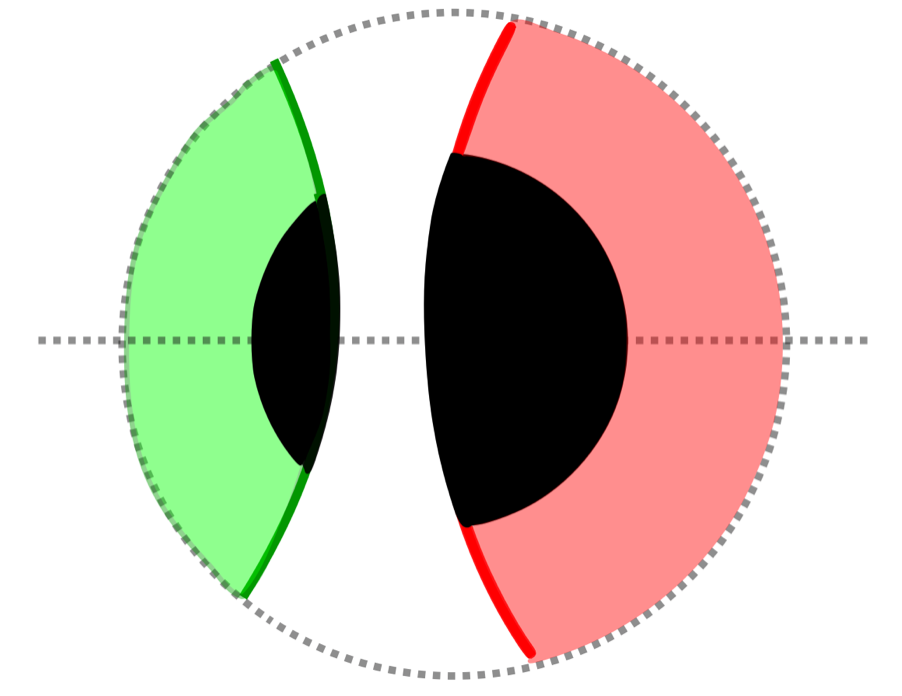
\includegraphics[width=0.5\textwidth]{figures/sigmasym.png}
    \caption{Schematic representation of $\left[\text{H}2,\text{H}2\right]$ solution. The horizontal broken line is the axis of reflection symmetry.}
    \label{symmetric geometry}
\end{figure}

\begin{figure}
    \centering
    \includegraphics[width=0.5\textwidth]{figures/kruskal.png}
    \caption{BTZ black hole in Kruskal-Szekeres coordinates. Only $u$ and $v$ coordinates are represented assuming spherical symmetry.}
    \label{Kruskal BTZ}
\end{figure}
